\subsection{Fading}\label{sc:fading}
%TODO: Forklar gerne "Intrinsic and extrinsic electronic noise set the signal to noise ratio (SNR) floor of the received signal"
The above plots all give a good estimate of the RF input power in a stationary clean environment with fixed-positioned nodes, but in case of a dynamic environment with obstacles, aspects like fading must be considered. Intrinsic and extrinsic electronic noise set the signal to noise ratio (SNR) floor of the received signal, but more expensive electronics can compensate for the former noise source, and if no mobile phones are at the track, it can lead to less of the latter noise source, however one would still 
experience RF input power drops at times in a dynamic environment.

\noindent The broadcasting behavior of the WSN causes constructive and destructive interference at the receiver, which can lead to deep fading. The phenomenon can occur when two or more, out of phase, adequate signals arrive at the receiver simultaneously leading to a critical destructive interference. Deep fading causes the signal strength to fall below the established noise floor, deeming the signal unreliable or unmeasurable. If a receiver has experienced a deep fade, depending on the time length or number of lost packages, it can either be categorized as a fast fade or a slow fade. More on these terms later. The fading is typically caused by reflection, diffraction or scattering of the signal, causing in line of sight (LOS) signal interfering with a none line of sight (NLOS) signals. When nodes move relative to each other it can not only cause interference, but also a change in behavior. An example of this is the Doppler fading, in which the signal tends to shift in frequency relative to the movement of the source and the sink node.
%TODO: Har ændret lidt i overstående, review gerne.

\subsubsection{Doppler Fading}
Following the standard IEEE\_802.15.4, it permits the telosb node to transmit in the ISM band at frequencies between $2.4$ and $2.4835 GHz$. Having 12 channels, $2 MHz$ wide and separated by $5 MHz$, the telosb allows a center frequency signal to shift $\pm 1 MHz$ while still being acknowledged by the receiving channel. If the signal shift the frequency more than $1 MHz$, the receiving node will simply filter out the signal and the packet will be lost. The sign of the shift in frequency varies if the distance between the source and the sink is increasing or decreasing. We will have a changing position of the runner relative to the base station at different speeds due to the track shape, so an investigation of the effects was made.

\noindent The distance between a packet, every quarter of a second, covered by a runner, running at $12kph$, was calculated closest and furthest on the track relative to the base station. The runner is running circular, but the change in distance experienced by the base station will by a straight line leading to Doppler frequency found at different speeds relative to track position. The results showed a $29.698Hz$ frequency shift at the end of the track, while at the top of the track a $26.773Hz$ shift happened. Since the telosb has a buffer of $1MHz$, the results put our misgivings about Doppler fading to rest. For the sake of scalability and flexibility, a extreme case was also calculated for the system: Had the runner been running at approximately $50000kph$, Doppler fading would have been an issue. Given the calculated results, the project is solely focusing on fast and slow fading as simulated instead. See appendix 2 for Doppler calculations.
%TODO: Ref appendix.

\subsubsection{Fast fading and slow fading}%TODO Is this how we want appendix? (footnote)
%TODO: Footnote explaing busty bit errors.
Busty bit errors at the receiver is often measured in clusters with different duration or length. Fast fading clusters are typically in the range of tens to hundreds of milliseconds, before the received signal again is adequate, while slow fading clusters are in the range of tens of seconds to minutes. Fast fading and slow fading are both by-products of the broadcasting behavior of the nodes. While no clean separation can be made between the two, slow fading is referred to as a shadowing effect and fast fading can be simplified to reflection, e.g. a signal at $2.4GHz$ will have a wavelength of $12.5cm$, given an opposite phased signal every $12.5cm$. If the $2.4GHz$ LOS signal travels $1m$ to the sink and the NLOS signal travels $1.125m$ to the sink, they would cancel each other out.

\noindent The calculations of the reflected fading also must consider the directivity of the antenna, since the signal strength also varies at different angles from the source. An antenna with high directivity will not have a full cancellation at the sink, since the LOS signal will have a higher amplitude than the NLOS signal. The drop-in signal strength can be estimated to around $30-40dB$ ($60-70dBm$)\footnote{Appendix: 1, page 92} and these are the values for both slow and fast fading chosen for the simulations in this project. Slow fading can represent diffraction and scattering of the signal from objects in between source and sink, e.g. more runners on the track or a photographer taking images along the route. The slow fading is modeled as a random stochastic variable with a showing variance visualized through a log-normal fading plot. Given a shadowing variance of $2.22dBm$ and probability of occurrence at $10\%$ for both fast and slow fading, fast fading effect is simulated to last $333 ms$ while slow fading is simulated to last $14s$. Figure \ref{fig:logpathReceivedSignal_baseStation_baseOnly} plots the base station's RF input power including fading and \ref{fig:binaryDeepFading_baseStation_baseOnly} plots the binary, received or lost package, output of the base station. Figure \ref{fig:logpathReceivedSignal_combinedStations_baseOnly} plots the RF input power of the stations combined including fading and \ref{fig:binaryDeepFading_combinedStations_baseOnly} plots the binary output of the stations combined. Figure \ref{fig:logpathReceivedSignal_combinedStations_allStations} and \ref{fig:binaryDeepFading_combinedStations_allStations} show a plot of combined stations, but with all three station signals being victims of individual fading patterns. 

%Figure 7, 8 and 9
\begin{figure}[h]
	\centering
	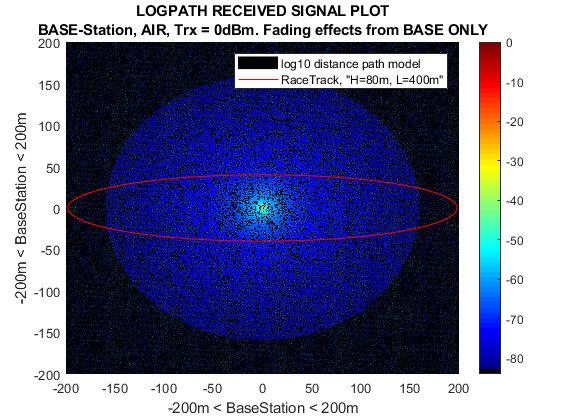
\includegraphics[width=\linewidth]{theory/fading/fig/logpathReceivedSignal_baseStation_baseOnly.png}
	\caption{Base Station RF input power plot after base station experiencing fading}
	\label{fig:logpathReceivedSignal_baseStation_baseOnly}
\end{figure}

\begin{figure}[h]
	\centering
	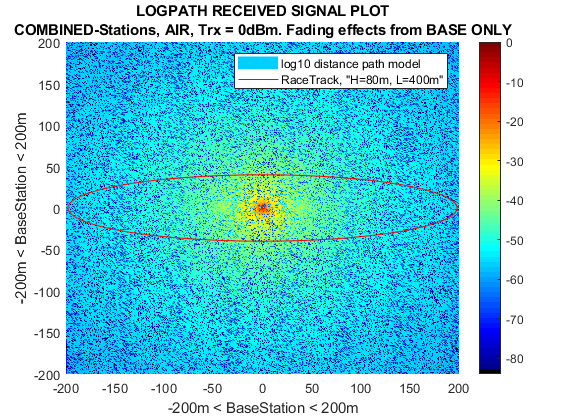
\includegraphics[width=\linewidth]{theory/fading/fig/logpathReceivedSignal_combinedStations_baseOnly.png}
	\caption{Combined Stations RF input power plot after base station experiencing fading}
	\label{fig:logpathReceivedSignal_combinedStations_baseOnly}
\end{figure}

\begin{figure}[h]
\centering
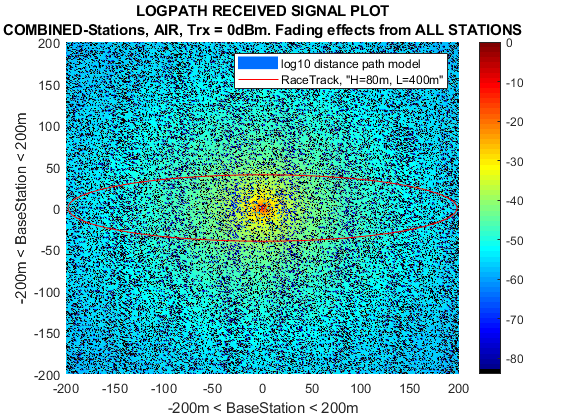
\includegraphics[width=\linewidth]{theory/fading/fig/logpathReceivedSignal_combinedStations_allStations.png}
\caption{Combined Stations RF input power plot after all stations experiencing fading}
\label{fig:logpathReceivedSignal_combinedStations_allStations}
\end{figure}

\begin{figure}[h]
	\centering
	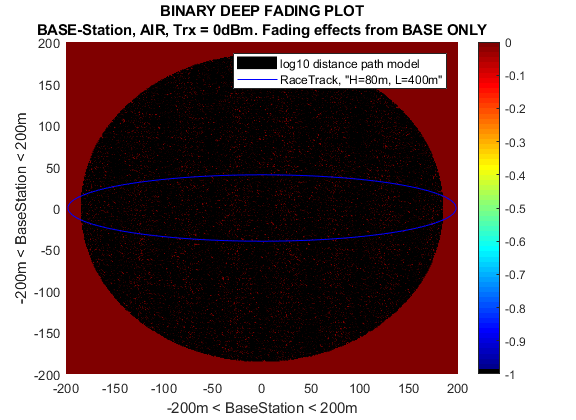
\includegraphics[width=\linewidth]{theory/fading/fig/binaryDeepFading_baseStation_baseOnly.png}
	\caption{Base Station Deep fading plot after base station experiencing fading}
	\label{fig:binaryDeepFading_baseStation_baseOnly}
\end{figure}

\begin{figure}[h]
	\centering
	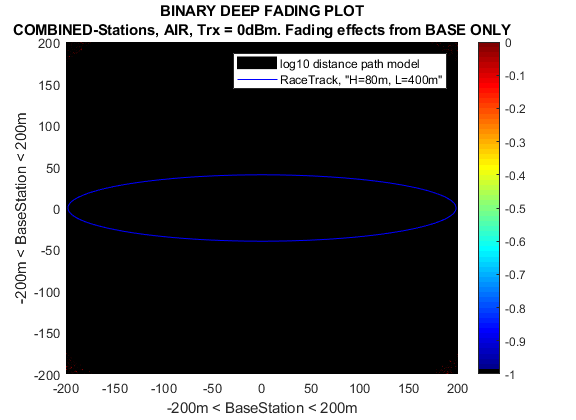
\includegraphics[width=\linewidth]{theory/fading/fig/binaryDeepFading_combinedStations_baseOnly.png}
	\caption{Combined Stations Deep fading plot after base station experiencing fading}
	\label{fig:binaryDeepFading_combinedStations_baseOnly}
\end{figure}

\begin{figure}[h]
	\centering
	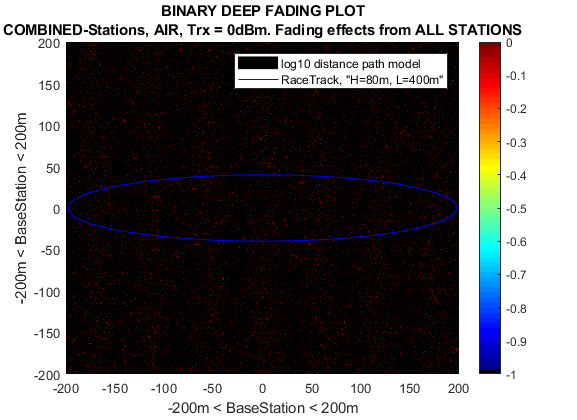
\includegraphics[width=\linewidth]{theory/fading/fig/binaryDeepFading_combinedStations_allStations.png}
	\caption{Combined Stations Deep fading plot after all stations experiencing fading}
	\label{fig:binaryDeepFading_combinedStations_allStations}
\end{figure}

